\documentclass[letter, pt=10]{scrartcl}

% Use UTF-8 encoding
\usepackage[utf8]{inputenc}
\usepackage{graphicx}
\usepackage{subfig}
\usepackage[margin=0.5in]{geometry}

\title{Final Project}
\author{Tobias Gerken}
\date{\today}


\begin{document}

\maketitle

\emph{\textbf{Disclamer:} This work uses generated toy data to visualize the effect of sampling size on our ability to detect climate change from data. This is overly simplified! }

\section{Abstract}
We use Bayesian ANOVA to explore the effect of sampling size on detecting the effects of climate change on global and local surface temperatures. We find that comparatively small sampling sizes are needed to detect statistically significant differences between mean temperatures from 1951-1980 and today's temperatures. However, this is an overly simplified analysis 


\section{Introduction}
A recent work by Sippel et al. in Nature Climate Change \cite{Sippel} demonstrated through statistical analysis that the effects of climate change are now detectable from  air temperature measurements every day. In other words, on any given day there is at least one place on Earth that is unusually warm compared to historic climate. 
Figure~\ref{fig:hist} (adapted from the paper) shows a comparison of daily temperature anomalies between today's climate and a historic reference climate.

\begin{figure}[h!]
    \centering
    \subfloat{{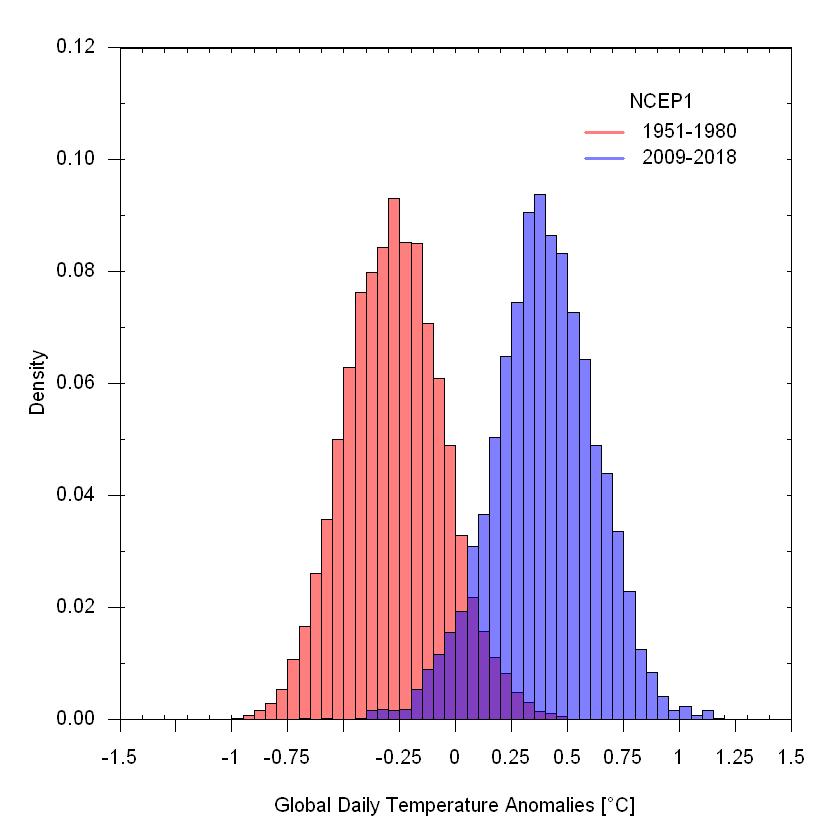
\includegraphics[width=5cm]{../Figures/TGlobal.png} }}%
    \qquad
    \subfloat{{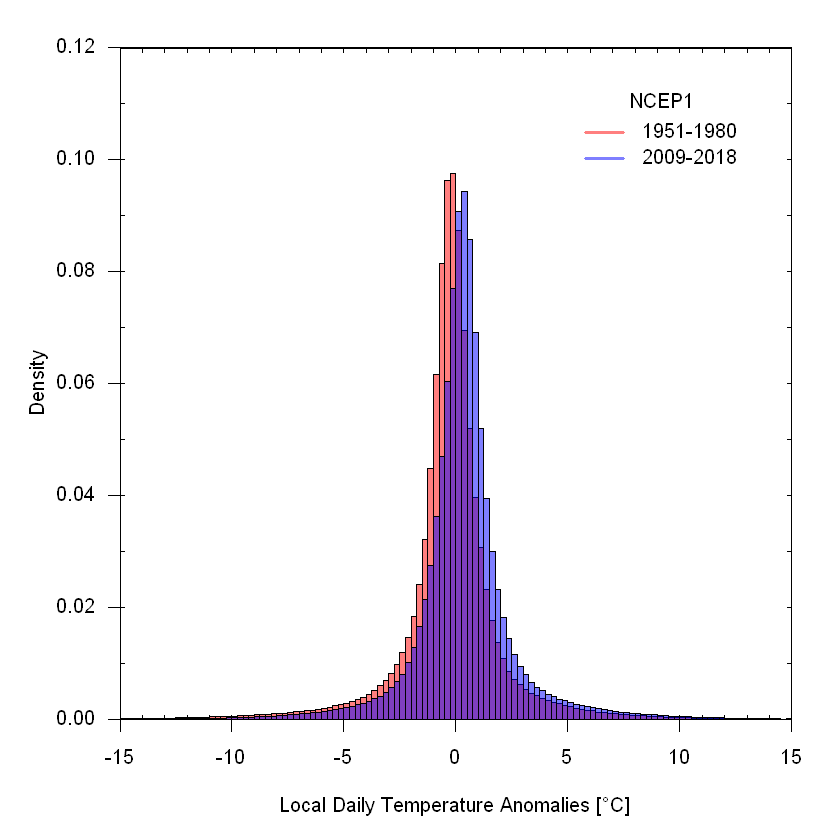
\includegraphics[width=5cm]{../Figures/TLocal.png} }}%
    \caption{Global and local surface temperature anomaly distribution for climate periods of 1951-1980 (referred to as \emph{early}) and 2009-2018 (today) compared to 1979-2005. Figure is adapted from Sippel et al. (2019, Nature Climate Change)}%
    \label{fig:hist}%
\end{figure}

Based on this data we perform ANOVA analysis to determine whether we can find significant differences in temperature distributions between 1951-1980 and today (2009-2018). Temperatures are expressed as anomalies, which means that the (1979-2005) means are subtracted and annual cycles are removed.  

\section{Data}
 Due to the amount of data involved and time constraints we generate data based on the paper by Sippel et al. They distributed the data from Figure~1, which is adapted from their paper (https://data.iac.ethz.ch/Sippel\_et\_al\_2019\_DailyDetection). The fact that this paper has undergone peer-review increases our confidence that this data is reliable.

The underlying data is based on the NOAA's NCEP/NCAR Reanalysis 1 \cite{NCEP} a global data-set of temperature data. While reanalysis data is not perfect, reanalysis data is extensively validated against observations.  

Given the fact that we only have probability density function of temperature anomalies, we generate the data-set by randomly sampling the density distribution. For the case of global average temperature, this is akin to randomly selecting a day and taking a single measurement of global mean temperature (and subtracting the mean). For the local surface temperature distribution, this is akin to taking a single measurement at a single location on the land surface, while similarly subtracting the mean.

This results in 4 groups of temperature data: (1) $T_{\mathrm{Early,Global}}$, (2) $T_{\mathrm{ Today,Global}}$, (3) $T_{\mathrm{Early,Local}}$, (4) $T_{\mathrm{Today,Local}}$, we use for further analysis.

\section{Modeling Approach}
A one-way ANOVA is performed on the data-set in order to establish whether there are a statistically significant difference in global and local temperature distributions between today and the earlier 20th century period. 

Using RJAGS v4.2 (https://sourceforge.net/projects/mcmc-jags/files/rjags/) we set up a linear model to estimate the mean of the distributions. Based on the central limit theorem we expect our model to follow a normal distribution with means $\mu$ using a normal prior for $\mu$ and gamma prior for $\sigma$. We use fairly non-informative priors for the prior normal ($\sigma = 10^6$) and gamma distributions (effective sample size = 5). We also allow $\sigma$ to vary independent between groups there is no reason to assume that all groups have the same standard deviation. 

The resulting model string in JAGS is:
%
\begin{verbatim}
mod_string = " model {
    for (i in 1:length(y)) {
        y[i] ~ dnorm(mu[grp[i]], prec)
    }
    
    for (j in 1:3) {
        mu[j] ~ dnorm(0.0, 1.0/1.0e6)
    }
    
    prec ~ dgamma(5/2.0, 5*1.0/2.0)
    sig = sqrt( 1.0 / prec )
} "
\end{verbatim}

The initial model is run using 3 Marcov Chains and we discard the first 3000 iterations and then run a further 5000 iterations each, resulting in a total of 15000 samples. 

We repeat this analysis for sample sizes of (5, 10,50,100,200,300,400,500,600,700,800,900,1000, 5000, 10000) for each group. Given the random sampling from the initial distribution, we assess the stability of results by repeating the entire analysis 50 times (i.e. this results in 50 estimates of $\mu$ for each group for each sample size). 

\section{Model Evaluation}
\sloppy
A visual inspection of the Marcov Chains suggests convergence of the runs and well behaved density distributions of $\mu$ and $\sigma$ values. Similarly, residual analysis suggests slight variation in $\sigma$ between present and earlier period, which is taken into account by the model. A q-q plot of the residuals does not show any apparent issues. Note that these plots can be found in the associated notebook on Github \\ (https://github.com/TobGerken/BayesianStats). 
\fussy
Regarding auto-correlation and effective sample size: It is important to realize that the data we generated for this work is free of autocorrelation, which is not the case for real world data, such that effective sample sizes are large. The effect of this is discussed later. I don't have space to show the results, but a model with a single variance fits the data less well!
 
\subsection{Results}

ANOVA results for 10000 samples show that for both local and global temperature distributions we have a probability of $>0.999$ that today's temperatures are warmer than temperatures of the earlier 20th century (Figure~\ref{fig:result}), which is in line with our understanding of anthropogenic climate change. We also find that using global mean temperatures rather than local temperatures we are able to detect this difference using a fairly small sample size of about 50 observations from each group, while for local observations $\sim$ 500 temperature observations are needed. We also see that for smaller sample sizes the effect of the random sampling from the underlying temperature distributions becomes important. 

\begin{figure}[h!]
    \centering
    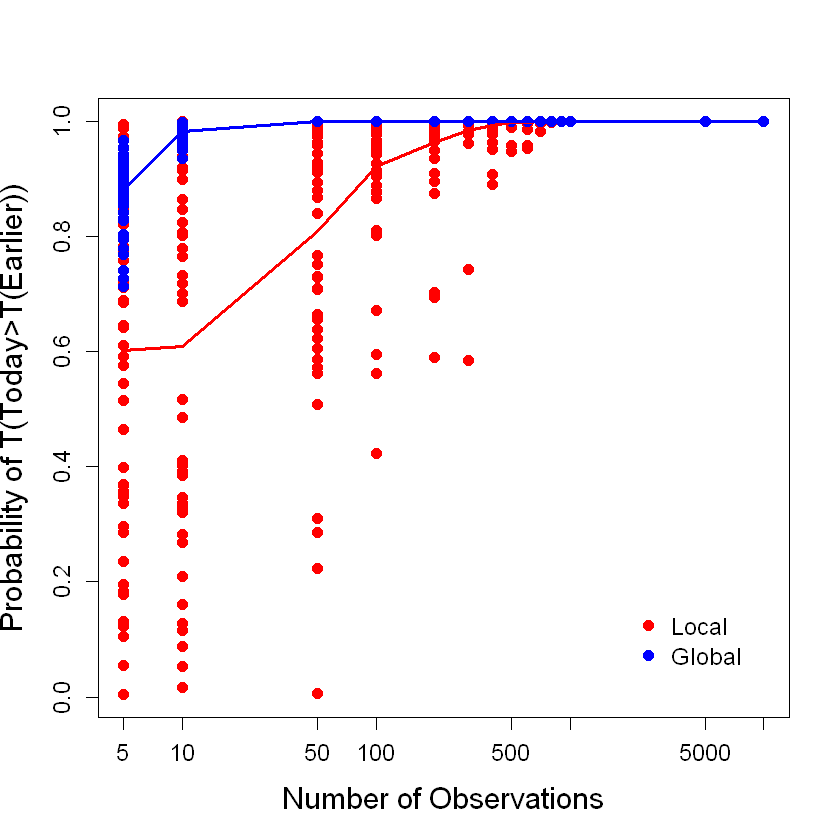
\includegraphics[width=6cm]{../Figures/Significance.png} %
    %\qquad
    %\subfloat{{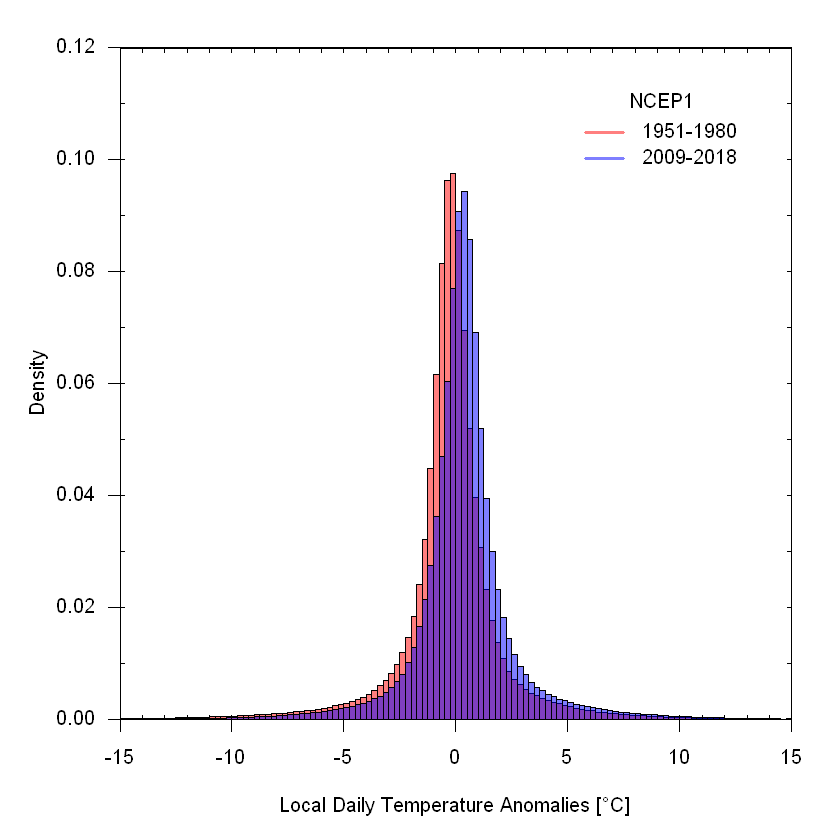
\includegraphics[width=5cm]{../Figures/TLocal.png} }}%
    \caption{Probability of detecting the effects of global climate change as a function of sample size. Each dot represents results of a ANOVA for a sample of points, while lines give the mean for each sample size.}%
    \label{fig:result}%
\end{figure}

The effect of random sampling from the underlying global temperature distribution can also be explained by modeled $\mu$-values in the ANOVA (Figure~\ref{fig:means}). For example we can see that for local temperature observations, we need about 500 samples each for the resulting posterior $\mu$ values to unmix (blue and cyan dots), while this unmixing happens at much smaller sample sizes. Note that while the means for each bin (dashed lines) start to approach the true mean global temperatures (horizontal dashed lines), there is still a large amount of variation between individual realizations, which indicates much higher numbers of temperature measurements are needed to estimate global mean temperatures themselves.   

\begin{figure}[h!]
    \centering
    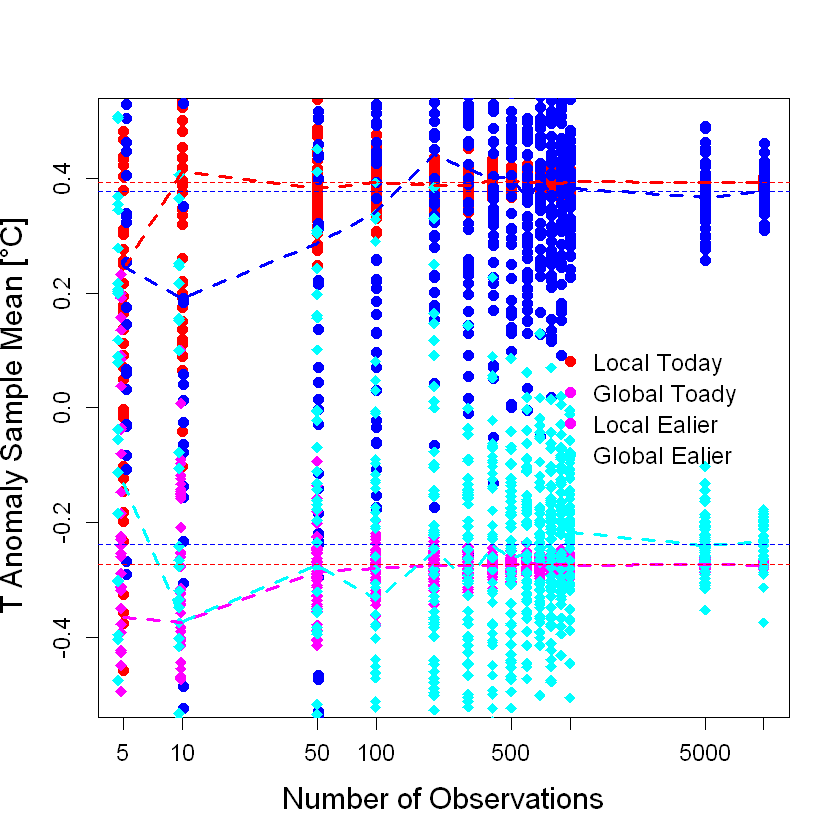
\includegraphics[width=6cm]{../Figures/Means.png} %
    %\qquad
    %\subfloat{{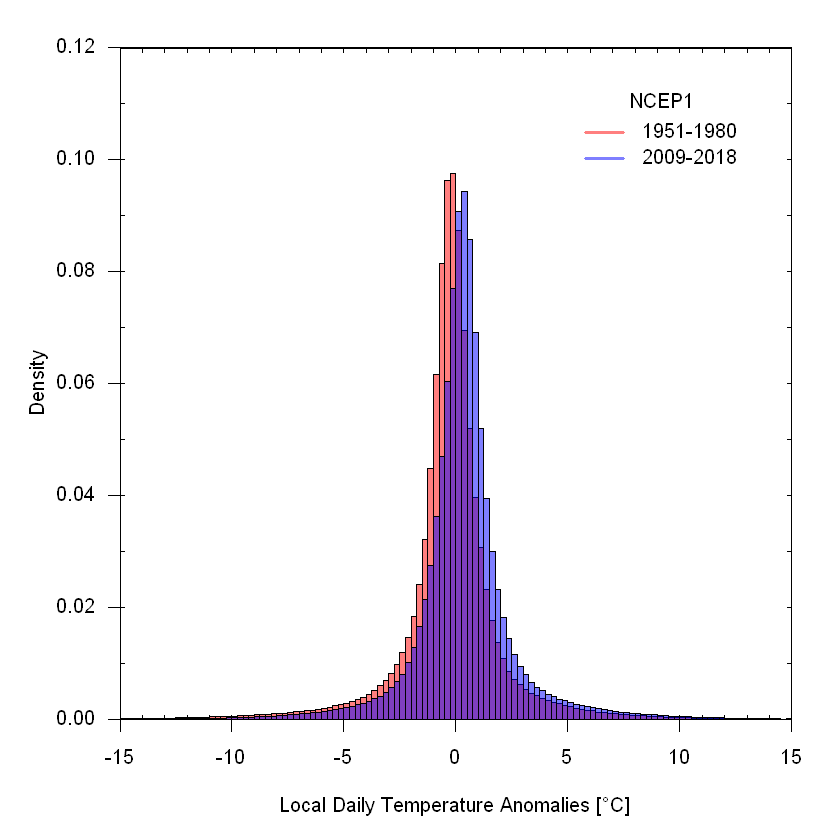
\includegraphics[width=5cm]{../Figures/TLocal.png} }}%
    \caption{Distribution of posterior $\mu$-values (dots) and their respective means (dashed lines) compared to true means (horizontal lines). Underling data from ANOVA results in Figure 3.}%
    \label{fig:means}%
\end{figure}

\subsubsection{Discussion}
Our results indicate that it is indeed possible to show statistically that global temperatures have changes using a reduced number of temperature observations. However, this analysis has several shortcomings. For example, we have relied on the total \emph{true} distribution of temperatures for our sampling, which means that all the work on sample collection, quality control etc has already been conducted. 

Similarly, we have randomized our sampling, which has removed autocorrelations from the dataset, while most real temperature data will have high autocorrelations. 

In summary, this should only be considered a toy example conducted to play around with Bayesian statistical methods. 

%\bibliographystyle{apalike}
%\begin{thebibliography}{9}

%\bibitem{Sippel}
%Sippel, S., Meinshausen, N., Fischer, E.M., Székely, E., Knutti, R., 2020. Climate change %now detectable from any single day of weather at global scale. Nat. Clim. Chang. 10, 35–41. https://doi.org/10.1038/s41558-019-0666-7

%\bibitem{NCEP}
NCEP/NCAR Reanalysis 1: https://www.esrl.noaa.gov/psd/data/gridded/data.ncep.reanalysis.html

%\end{thebibliography}

\end{document}